\section{Transformée de \nom{Laplace}} 
\label{transformee_laplace}

\todoarmand{Un thème assez développé sur la transformée de Laplace : \url{https://cahier-de-prepa.fr/ecg2-saintlouis/download?id=289}
}

La transformation de \nom{Laplace} généralise la transformation de \nom{Fourier} qui est également utilisée pour résoudre les équations différentielles : contrairement à cette dernière, elle tient compte des conditions initiales et peut ainsi être utilisée en théorie des vibrations mécaniques ou en électricité dans l'étude des régimes forcés sans négliger le régime transitoire. De manière générale, ses propriétés vis-à-vis de la dérivation permettent un traitement plus simple de certaines équations différentielles, et elle est de ce fait très utilisée en automatique.

Dans ce type d'analyse, la transformation de \nom{Laplace} est souvent interprétée comme un passage du domaine temps, dans lequel les entrées et sorties sont des fonctions du temps, dans le domaine des fréquences, dans lequel les mêmes entrées et sorties sont des fonctions de la \say{ fréquence } (complexe) $p$. Ainsi, il est possible d'analyser simplement l'effet du système sur l'entrée pour donner la sortie en matière d'opérations algébriques simples (cf. théorie des fonctions de transfert en électronique ou en mécanique). 

\begin{defi}[Fonction causale]
\begin{comment}
\begin{itemize}
    \item On appelle \definir{fonction causale} une fonction définie sur $\R$ dont le support est borné à gauche en $0$ \emph{i.e.} $f$ est nulle pour tout $x < 0$. 
    \item On appelle fonction causale toute fonction définie sur $\R$, nulle sur $\interoo{-\infty}{0}$ et continue par morceaux sur $\interfo{0}{+\infty}$.
\end{itemize}
\end{comment}
Une fonction $f$ définie sur $\R$ est une \definir{fonction causale} si elle est continue par morceaux et nulle sur $\interfo{0}{+\infty}$.
\end{defi}


\begin{remarque}
La fonction de \nom{Heaviside} est définie par $H = \indicatrice{\Rp}$. Étant donnée une fonction $g$ non causale, la fonction $f = H \times g$ est une fonction causale.
\end{remarque}

\begin{defi}[Transformée de \nom{Laplace}]
    Soit $f$ une fonction causale. On note, lorsqu'elle converge, 
    $$\mathscr{L}(f)(p) \defeq \int_{0}^{+ \infty} \e^{-pt} f(t) \d t.$$
    La fonction $\mathscr{L}(f)$ est la \definir{transformée de \nom{Laplace} de $f$}.
\end{defi}

\marginnote[0cm]{Sources : \cite{exos_oraux} + \cite{acamanes} (Exercice cerise Ch. 12)}
% \underline{Démonstration du théorème de la valeur finale:}
% \begin{itemize}
    % \item Généralisation classique du théorème des bornes $\leadsto$ $f$ est bornée
    % \item Changement de variable: $\varphi: u \mapsto \frac{u}{p}$
    % \item Caractérisation séquentielle de la limite
    % \item Théorème de convergence dominée
% \end{itemize}

\todoinline{Pointer vers CCP - MP - 2011}

%-----------
\subsection{Exemples de transformées de \nom{Laplace}}

\begin{exercice}
Soient $\lambda \in \C$ et $n \in \N$. Pour chacune des fonctions suivantes, déterminer leur transformée de~\nom{Laplace} en précisant le domaine de définition :
\begin{tasks}(3)
    \task $t \mapsto 1$.
    \task $t \mapsto \e^{\lambda t}$.
    \task $t \mapsto t^n$.
\end{tasks}
\end{exercice}

\begin{solution}
\begin{reponses}
\item La fonction $t \mapsto \e^{-pt}$ est intégrable sur $\Rp$ si et seulement si $p > 0$. Alors,
\[
\forall\, p > 0,\,
\mathscr{L}(f)(p) = \int_0^{+\infty} \e^{-pt} \d t = \frac{1}{p}.
\]

\item La fonction $t \mapsto \e^{-(\lambda-p)t}$ est intégrable sur $\Rp$ si et seulement si $p > \Reel(\lambda)$. Alors,
\[
\mathscr{L}(f)(p)
= \int_0^{+\infty} \e^{-(p-\lambda)t} \d t
= \frac{1}{p-\lambda}.
\]

\item Soit $n \in \Ne$ et $\fonctionligne[f_n]{t}{t^n \e^{-pt}}$.
\begin{itemize}
\item La fonction $f_n$ est continue sur $\Rpe$.
\item Si $p > 0$, alors $f(t) = o_{+\infty}(1/t^2)$ et $f$ est intégrable sur $\Rpe$.

Si $p \leqslant 0$, alors $\lim_{+\infty} f = +\infty$ et $f$ n'est pas intégrable sur $\Rpe$.
\end{itemize}
Ainsi, $f_n$ est intégrable si et seulement si $p > 0$. Une récurrence classique avec des intégrations par parties permet de montrer que
\[
\mathscr{L}(f)(p) = \frac{n!}{p^{n+1}}.
\]
\end{reponses}
\end{solution}

\todoarmand{Résoudre problème avec adjustbox{valign=c}}
\todoarmand{Ajouter les derniers graphes}
\begin{table}[h!]
    \centering
    % \renewcommand{\arraystretch}{3.0}
    % \setlength{\tabcolsep}{0.5em}
    \SetTblrInner{rowsep=3pt}
    \def\colplot{cyan}
    \def\a{-0.3}
    \def\b{3.8}
    \def\xmin{-0.1}
    \def\xmax{4.1}
    \def\amp{1}
    \def\puls{8}
    \def\damp{0.6}
    \def\samp{200}
    \begin{tblr}{
        colspec = {|cc|cc|}
    }
        \hline
        $f(t) \mathbf{1}_{t > 0}$ & $f(t)$ & $\mathcal{L}(f)(p)$ & \\ \hline\hline
        % Row 2
        % \adjustbox{valign=c}{%
            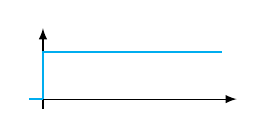
\begin{tikzpicture}[scale=0.6]
                \draw[-latex] (\xmin,0) -- (\xmax,0);
                \draw[-latex] (0,-0.2) -- (0,1.5);
                \draw[\colplot, thick, domain=\a:0] plot (\x, 0);
                \draw[\colplot, thick] (0,0) -- (0,1) -- (\b,1);
            \end{tikzpicture}%
        % } 
        & $ A $ & $\displaystyle \frac{A}{p} $ & 
        % \adjustbox{valign=c}{%
            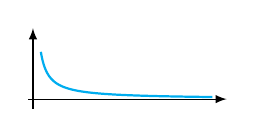
\begin{tikzpicture}[scale=0.6]
                \draw[-latex] (\xmin,0) -- (\xmax,0);
                \draw[-latex] (0,-0.2) -- (0,1.5);
                \draw[\colplot, thick, domain=1/6:\b, samples=\samp] plot (\x, {1/(6*\x)});
            \end{tikzpicture}%
        % }
        \\ \hline

        % Row 3
        % \adjustbox{valign=c}{%
            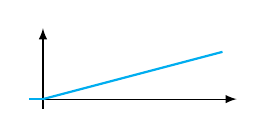
\begin{tikzpicture}[scale=0.6]
                \draw[-latex] (\xmin,0) -- (\xmax,0);
                \draw[-latex] (0,-0.2) -- (0,1.5);
                \draw[\colplot, thick, domain=\a:0] plot (\x, 0);
                \draw[\colplot, thick] (0,0) -- (\b,1);
            \end{tikzpicture}%
        % } 
        & $ a\,t$ % \cdot u(t) $ 
        & $\displaystyle \frac{a}{p^2} $ & 
        % \adjustbox{valign=c}{%
            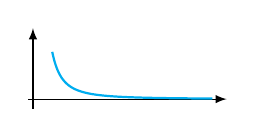
\begin{tikzpicture}[scale=0.6]
                \draw[-latex] (\xmin,0) -- (\xmax,0);
                \draw[-latex] (0,-0.2) -- (0,1.5);
                \draw[\colplot, thick, domain=0.40824829046:\b, samples=\samp] plot (\x, {1/(6*\x^2)});
            \end{tikzpicture}%
        % } 
        \\ \hline

        % Row 4
        % \adjustbox{valign=c}{%
            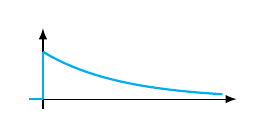
\begin{tikzpicture}[scale=0.6]
                \draw[-latex] (\xmin,0) -- (\xmax,0);
                \draw[-latex] (0,-0.2) -- (0,1.5);
                \draw[\colplot, thick, domain=\a:0] plot (\x, 0);
                \draw[\colplot, thick] (0,0) -- (0,\amp);
                \draw[\colplot, thick, domain=0:\b] plot (\x, {\amp*exp(-\damp*\x)});
            \end{tikzpicture}%
        % }
        & $ \mathrm{e}^{-at}$ % $ \cdot u(t) $ 
        & $\displaystyle \frac{1}{p + a} $ & 
        % \adjustbox{valign=c}{%
            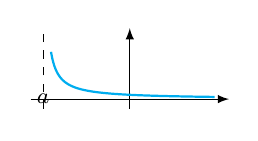
\begin{tikzpicture}[scale=0.6]
                \draw[-latex] (\xmin,0) -- (\xmax,0);
                \draw[-latex] (2,-0.2) -- (2,1.5);
                \draw[dashed] (1/6,-0.2) -- (1/6,1.5);
                \node at (1/6, 0) {\footnotesize $a$};
                \draw[\colplot, thick, domain=1/3:\b, samples=\samp] plot (\x, {1/(6*(\x-1/6))});
            \end{tikzpicture}%
        % } 
        \\ \hline

        % Row 5
        % \adjustbox{valign=c}{%
            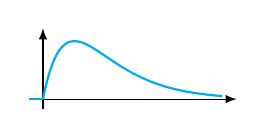
\begin{tikzpicture}[scale=0.6]
                \draw[-latex] (\xmin,0) -- (\xmax,0);
                \draw[-latex] (0,-0.2) -- (0,1.5);
                \draw[\colplot, thick, domain=\a:0] plot (\x, 0);
                \draw[\colplot, thick, domain=0:\b, samples=\samp] plot (\x, {5*\x*exp(-1.5*\x)});
            \end{tikzpicture}%
        % }
        & $ t\, \mathrm{e}^{-at}$ % $ \cdot u(t) $ 
        & $\displaystyle \frac{1}{(p + a)^2} $ & 
        % \adjustbox{valign=c}{%
            \begin{tikzpicture}[scale=0.6]
                \draw[-latex] (\xmin,0) -- (\xmax,0);
                \draw[-latex] (0,-0.2) -- (0,1.5);
            \end{tikzpicture}%
        % } 
        \\ \hline

        % Row 6
        % \adjustbox{valign=c}{%
            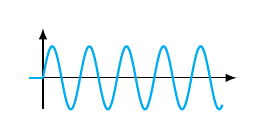
\begin{tikzpicture}[scale=0.6]
                \draw[-latex] (\xmin,0) -- (\xmax,0);
                \draw[-latex] (0,-0.65) -- (0,1.05);
                \draw[\colplot, thick, domain=\a:0] plot (\x, 0);
                \draw[\colplot, thick, domain=0:\b, samples=\samp] plot (\x, {\amp/1.5*sin(\puls*\x r)});
            \end{tikzpicture}%
        % } 
        & $ \sin(\omega t)$ % $ \cdot u(t) $ 
        & $\displaystyle \frac{\omega}{p^2 + \omega^2} $ & 
        % \adjustbox{valign=c}{%
            \begin{tikzpicture}[scale=0.6]
                \draw[-latex] (\xmin,0) -- (\xmax,0);
                \draw[-latex] (0,-0.65) -- (0,1.05);
            \end{tikzpicture}%
        % }
        \\ \hline

        % Row 7
        % \adjustbox{valign=c, width=0.22\textwidth}{%
            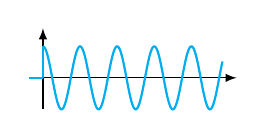
\begin{tikzpicture}[scale=0.6]
                \draw[-latex] (\xmin,0) -- (\xmax,0);
                \draw[-latex] (0,-0.65) -- (0,1.05);
                \draw[\colplot, thick, domain=\a:0] plot (\x, 0);
                \draw[\colplot, thick] (0,0) -- (0,\amp/1.5);
                \draw[\colplot, thick, domain=0:\b, samples=\samp] plot (\x, {\amp/1.5*cos(\puls*\x r)});
            \end{tikzpicture}%
        % } 
        & $ \cos(\omega t)$ % $ \cdot u(t) $ 
        & $\displaystyle \frac{p}{p^2 + \omega^2} $ & 
        % \adjustbox{valign=c}{%
            \begin{tikzpicture}[scale=0.6]
                \draw[-latex] (\xmin,0) -- (\xmax,0);
                \draw[-latex] (0,-0.65) -- (0,1.05);
            \end{tikzpicture}%
        % }
        \\ \hline

        % Row 8
        % \adjustbox{valign=c}{%
            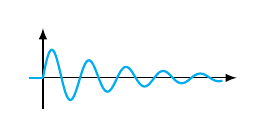
\begin{tikzpicture}[scale=0.6]
                \draw[-latex] (\xmin,0) -- (\xmax,0);
                \draw[-latex] (0,-0.65) -- (0,1.05);
                \draw[\colplot, thick, domain=\a:0] plot (\x, 0);
                \draw[\colplot, thick, domain=0:\b, samples=\samp] plot (\x, {\amp/1.5*exp(-\damp*\x)*sin(\puls*\x r)});
            \end{tikzpicture}%
        % }
        & $ \mathrm{e}^{-at} \sin(\omega t)$ % $ \cdot u(t) $ 
        & $\displaystyle \frac{\omega}{(p + a)^2 + \omega^2} $ & 
        % \adjustbox{valign=c}{%
            \begin{tikzpicture}[scale=0.6]
                \draw[-latex] (\xmin,0) -- (\xmax,0);
                \draw[-latex] (0,-0.65) -- (0,1.05);
            \end{tikzpicture}%
        % }
        \\ \hline

        % Row 9
        % \adjustbox{valign=c}{%
            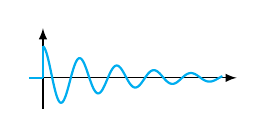
\begin{tikzpicture}[scale=0.6]
                \draw[-latex] (\xmin,0) -- (\xmax,0);
                \draw[-latex] (0,-0.65) -- (0,1.05);
                \draw[\colplot, thick, domain=\a:0] plot (\x, 0);
                \draw[\colplot, thick] (0,0) -- (0,\amp/1.5);
                \draw[\colplot, thick, domain=0:\b, samples=\samp] plot (\x, {\amp/1.5*exp(-\damp*\x)*cos(\puls*\x r)});
            \end{tikzpicture}%
        % }
        & $ \mathrm{e}^{-at} \cos(\omega t)$ % $ \cdot u(t) $ 
        & $\displaystyle \frac{p + a}{(p + a)^2 + \omega^2} $ & 
        % \adjustbox{valign=c}{%
            \begin{tikzpicture}[scale=0.6]
                \draw[-latex] (\xmin,0) -- (\xmax,0);
                \draw[-latex] (0,-0.65) -- (0,1.05);
            \end{tikzpicture}%
        % }
        \\ \hline
    \end{tblr}
    \caption{Tableaux des transformées de \textsc{Laplace} usuelles}
\end{table}

\begin{remarque}
À un changement de variable près, on reconnaît, pour la dernière transformée de \nom{Laplace}, la fonction Gamma d'\nom{Euler}.\marginnote[0pt]{\href{subsec:FonctionGammaEuler}{\faLink~Fonction Gamma d'\nom{Euler}}}
\end{remarque}


\begin{theo}
\begin{enumerate}
\item Si la fonction $f$ est bornée, alors $\mathscr{L}(f)$ est définie et de classe $\mathscr{C}^\infty$ sur $\Rpe$.

\item Si $\int_0^{+\infty} f(t) \d t$ converge, alors $\mathscr{L}(f)$ est définie sur $\Rp$.

\item Si $f$ est continue uniquement sur $\Rpe$ et qu'il existe $p_0 > 0$ tel que, pour pour tout $p > p_0$, la fonction $t \mapsto \e^{-p t} f(t)$ est intégrable sur $\Rp$, alors $\mathscr{L}(f)$ est définie et continue sur $\interoo{p_0}{+\infty}$.
\end{enumerate}
\end{theo}

\begin{demo}
\begin{enumerate}
\item La fonction $f$ est bornée par une constante $M$. On utilise le \theoremeutilise{théorème de dérivation sous le signe intégral}{thm:derivsousintegrale}. Notons $\fonctionligne[g]{(p, t)}{f(t) \e^{-pt}}$.
\begin{itemize}
\item Pour tout $t \in \Rpe$, la fonction $\fonctionligne[g(\,\cdot\,, t)]{p}{\e^{-p t} f(t)}$ est de classe $\mathscr{C}^\infty$ sur $\Rpe$ et
\[
\forall j \in \N,\quad \frac{\partial^j g}{\partial p^j} g(p, t) = (-1)^j t^j f(t) \e^{-pt}.
\]

\item Pour tout $p > 0$, la fonction $\fonctionligne[g(p,\,\cdot\,)]{t}{(-1)^j t^j \e^{-p t} f(t)}$ est continue sur $\interfo{0}{+\infty}$.

\item Soit $\tilde{p} > 0$. Alors, pour tout $p \geqslant \tilde{p}$,
\[
\abs{(-1)^j t^j f(t) \e^{-p t}} \leqslant M t^j \e^{- \tilde{p} t} M.
\]
De plus, la fonction $\fonctionligne[\phi_j]{t}{M t^j \e^{-\tilde{p} t}}$ est continue sur $\Rp$, et est négligeable devant $1/t^2$ en $+\infty$. Ainsi, $\phi_j$ est intégrable.
\end{itemize}
Ainsi, la transformée de \nom{Laplace} $\mathscr{L}(f)$ est de classe $\mathscr{C}^\infty$ sur $\Rpe$.

\item Lorsque $p = 0$, l'intégrale $\int_0^{+\infty} \e^{-0\cdot t} f(t) \d t$ converge par hypothèse et $\mathscr{L}(f)(0)$ est donc bien définie.

\medskip

Soit $p > 0$. Comme $f$ est continue, on note $\fonctionligne[F]{x}{\int_0^x f(t) \d t}$ sa primitive qui s'annule en $0$.

Par hypothèse, $F$ possède une limite finie en $+\infty$. Ainsi, d'après le théorème d'intégration par parties, les intégrales $\int_0^{+\infty} \e^{-p t} f(t) \d t$ et $\int_0^{+\infty} \e^{-p t} F(t) \d t$ sont de même nature.

Enfin, comme $F$ est continue sur $\Rp$ et admet une limite finie en $+\infty$, alors $F$ est bornée sur $\Rp$. Il existe donc une constante $M$ telle que
\[
\module{\e^{-p t} F(t)} \leqslant M \e^{-p t}.
\]
Ainsi, la fonction $t \mapsto \e^{-p t} F(t)$ est intégrable, donc $\int_0^{+\infty} \e^{-p t} F(t) \d t$ converge et $\mathscr{L}(f)(p)$ est bien définie.

\item Soit $\fonctionligne[g]{(p, u)}{f(u) \e^{-p u}}$.
\begin{itemize}
\item $\forall t \in \Rpe$, $g(\,\cdot\,, u)$ est continue sur $\interoo{p_0}{+\infty}$.
\item $\forall p > p_0$, $g(p, \cdot)$ est continue sur $\Rpe$.
\item Soit $\tilde{p} > p_0$. Pour tout $p \geqslant \tilde{p}$ et $t \in \Rpe$,
\[
\abs{\e^{-p t} f(t)} \leqslant \e^{- \tilde{p} t} \abs{f(t)}.
\]
De plus, la fonction $t \mapsto f(t) \e^{-\tilde{p} t}$ est intégrable sur $\Rpe$ par hypothèse.
\end{itemize}
D'après le \theoremeutilise{théorème de continuité sous le signe intégral}{thm:contsousintegrale}, la transformée $\mathscr{L}(f)$ est continue sur $\interoo{p_0}{+\infty}$.
\end{enumerate}
\end{demo}


%-----------
\subsection{Théorème de la valeur finale}

\begin{theo}[Théorème de la valeur finale]
On suppose qu'il existe un réel $\ell$ non nul tel que $\lim\limits_{x \to +\infty} f(x) = \ell$. Alors,
\[
\lim_{p\to 0} p\, \mathscr{L}(f)(p) = \ell.
\]
\end{theo}

\begin{exercice}
On se place sous les hypothèses du théorème.
\begin{questions}
\item Montrer que $\mathscr{L}(f)$ est définie sur $\Rpe$.

\item Montrer que $p \mathscr{L}(f)(p) = \int_0^{+\infty} \e^{-u} f\big(\frac{u}{p}\big) \d u$.

\item Montrer que, si $(p_n)$ est une suite de réels strictement positifs qui tend vers $0$, alors $\lim\limits_{n\to+\infty} p_n\, \mathscr{L}(f)(p_n) = \ell$.

\item Conclure.
\end{questions}
\end{exercice}

\begin{solution}
\begin{reponses}
\item Comme $f$ est continue sur $\Rp$ et possède une limite en $+\infty$, une généralisation classique du \theoremeutilise{théorème des bornes}{thm:bornes} assure que $f$ est bornée sur $\Rp$. Ainsi, d'après le théorème précédent, la transformée $\mathscr{L}(f)$ est bien définie sur $\Rpe$.

\item On effectue le changement de variable affine $\fonctionligne[\phi]{u}{\frac{u}{p}}$. Alors,
\[
p\, \mathscr{L}(f)(p) = \int_0^{+\infty} \e^{-u} f\mathopen{}\left(\frac{u}{p}\right) \d u.
\]

\item Posons $\fonctionligne[g_n]{u}{\e^{-u} f(u/p_n)}$.
\begin{itemize}
\item Pour tout $n \in \N$, la fonction $g_n$ est continue sur $\Rp$.

\item Soit $u > 0$. D'après les hypothèses sur la fonction $f$, $\lim\limits_{n\to+\infty} \e^{-u} f(u/p_n) = \e^{-u} \ell$. Ainsi, la suite de fonctions $(g_n)$ converge simplement sur $\Rpe$ vers $u \mapsto \e^{-u} \ell$.

\item Comme $f$ est bornée par une constante $M$, $\abs{g_n(u)} \leqslant M \e^{-u}$ et la fonction $u \mapsto \e^{-u}$ est intégrable sur $\Rpe$.
\end{itemize}
Ainsi, d'après le \theoremeutilise{théorème de convergence dominée}{thm:convdominee},
\[
\lim_{n\to+\infty} p_n\, \mathscr{L}(f)(p_n) = \ell \int_0^{+\infty} \e^{-u} \d u = \ell.
\]

\item En utilisant la \theoremeutilise{caractérisation séquentielle de la limite}{caracsequlimite},
\[
\lim_{p\to 0} p\, \mathscr{L}(f)(p) = \ell \quad \text{soit} \quad \mathscr{L}(f)(p) \sim_0 \frac{\ell}{p}.
\]
\end{reponses}
\end{solution}

%-----------
\subsection{Théorème de la valeur initiale}

\begin{theo}[Théorème de la valeur initiale]
On suppose que $f$ est continue sur $\Rpe$ et qu'il existe $p_0 > 0$ tel que, pour pour tout $p > p_0$, $t \mapsto \e^{-p t} f(t)$ est intégrable sur $\Rp$. On suppose de plus qu'il existe un réel $\ell$ tel que $\lim_{t\to0^+} f(t) = \ell$. Alors,
\[
\lim_{p\to+\infty} p\, \mathscr{L}(f)(p) = \ell.
\]
\end{theo}

\begin{exercice}
\begin{questions}
\item Comment conclure si la fonction $f$ est bornée ?
\end{questions}

On suppose dans la suite que $f$ n'est pas nécessairement bornée. Soit $\varepsilon > 0$.
\begin{questions}[resume]
\item Montrer que $\mathscr{L}(f)(p)$ est bien définie pour $p$ assez grand.

\item Montrer qu'il existe un réel $h$ tel que
\[
\int_0^h p \module{f(t) - \ell} \e^{-p t} \d t \leqslant \varepsilon.
\]

\item Montrer qu'il existe un réel $\tilde{p}$ et une constante $c$ tels que pour tout $p \geqslant \tilde{p}$,
\[
p \int_h^{+\infty} \module{f(t)} \e^{-p t} \d t
\leqslant c p\,\e^{-(p-\tilde{p}) h}.
\]

\item Conclure.
\end{questions}
\end{exercice}

\begin{solution}
\begin{reponses}
\item  Si la fonction $f$ est bornée, on peut appliquer la même méthode que pour le théorème de la valeur finale.

\item Comme $\lim_{t\to0^+} f(t) = \ell$, il existe $h > 0$ tel que
\[
\forall t \in \interof{0}{h},\quad \abs{f(t) - \ell} \leqslant \varepsilon.
\]
Ainsi,
\begin{align*}
\int_0^h p \abs{f(t) - \ell} \e^{-p t} \d t
&\leqslant \varepsilon\big(1 - \underbrace{\e^{-p h}}_{\geqslant 0}\big)
\leqslant \varepsilon
.
\end{align*}

\item Posons $\tilde{p} = p_0 + \frac{1}{2}$. Alors, pour $p \geqslant \tilde{p}$,
\begin{align*}
p \int_h^{+\infty} \module{f(t)} \e^{-p t} \d t
&= p \int_h^{+\infty} \module{f(t)} \e^{-(p - \tilde{p}) t - \tilde{p} t} \d t\\
&\leqslant p\, \e^{-(p-\tilde{p}) h} \int_h^{+\infty} \module{f(t)} \e^{- \tilde{p} t} \d t\\
&\leqslant c p\, \e^{-(p-\tilde{p}) h}.
\end{align*}

\item Finalement, en utilisant l'inégalité triangulaire et la relation de \nom{Chasles}, pour $p \geqslant \tilde{p}$,
\begin{align*}
\abs{p\, \mathscr{L}(f)(p) - \ell}
&\leqslant \int_0^{+\infty} p \abs{f(t) - \ell} \e^{-p t} \d t \\
&\leqslant \int_0^h p \abs{f(t) - \ell} \e^{-pt} \d t
+ p \int_h^{+\infty} \abs{f(t)} \e^{-p t} \d t
+ p \int_h^{+\infty} \abs{\ell} \e^{- p t} \d t \\
&\leqslant \varepsilon + c p\, \e^{-(p-\tilde{p})h} + \module{\ell} \e^{-p h}.
\end{align*}

Comme $\lim\limits_{p\to+\infty} \e^{-p h} = \lim\limits_{p\to+\infty} p\, \e^{-(p-\tilde{p})h} = 0$, pour $p$ assez grand,
\[
\abs{p\, \mathscr{L}(f)(p) - \ell}
\leqslant 3 \varepsilon.
\]

Ainsi, d'après la définition de la limite,
\[
\lim_{p\,\to+\infty} p\, \mathscr{L}(f)(p) = \ell.
\]
\end{reponses}
\end{solution}


%--------------
\subsubsection{Méthode de \nom{Laplace}}
\todoinline{Ajouter méthode de Laplace ? cf . Mines 2 - PC - 2017 - Un cas discret est traité, ici on traite un cas continu}

\todoinline{Phrase introductive - Voir Rouvière - Petit guide de calcul différentiel pour un théorème plus complet}

\begin{theo}{Méthode de Laplace}
Soient $f$ une fonction de classe $\mathscr{C}^2$ et intégrable sur $\Rp$. Alors,
\[
F(t) = \int_0^{+\infty} \e^{-t x^2} f(t) \d x
\sim_{t\to+\infty} \frac{\sqrt{\pi}}{2} \cdot \frac{f(0)}{\sqrt{t}}.
\]
\end{theo}

\begin{remarque}
Par rapport au théorème de la valeur initiale, la fonction $\e^{-t x}$ a été remplacée par $\e^{-t x^2}$. L'heuristique de la démonstration est identique, à savoir que dès que $t$ devient grand, seules les valeurs de $f$ proches de $0$ comptent. Une généralisation de ce résultat permet de retrouver la formule de \nom{Stirling}. 
\end{remarque}

\begin{exercice}
\begin{questions}
\item Montrer que $F$ est bien définie sur $\Rp$.

\item À l'aide d'un changement de variable et du théorème de convergence dominée, montrer que
\[
\lim_{t\to+\infty} \sqrt{t} \int_0^1 \e^{-t x^2} f(x) \d x = f(0) \int_0^{+\infty} \e^{-u^2} \d u.
\]

\item Montrer que
\[
\lim_{t\to+\infty} \sqrt{t} \int_1^{+\infty} \e^{-t x^2} f(x) \d x = 0.
\]

\item Conclure.
\end{questions}
\end{exercice}

\begin{demo}
\begin{reponses}
\item Comme $\module{\e^{-t x^2} f(t)} \leq \module{f(t)}$, la fonction $F$ est bien définie.

\item Comme la fonction $f$ est continue sur $\interff{0}{1}$, elle est bornée par une constante $M$ sur ce segment. Alors, en utilisant le changement de variable affine $u \mapsto u/\sqrt{t}$,
\begin{align*}
\int_0^1 \e^{-t x^2} f(x) \d x
&= \int_0^{\sqrt{t}} \frac{\e^{-u^2}}{\sqrt{t}} f\left(\frac{u}{\sqrt{t}}\right) \d u\\
&= \frac{1}{\sqrt{t}} \int_0^{+\infty} \e^{-u^2} f\left(\frac{u}{\sqrt{t}}\right) \indicatrice{\interff{0}{\sqrt{t}}}(u) \d u.
\end{align*}
En utilisant une majoration par $u \mapsto M \e^{-u^2}$, le théorème de convergence dominée permet de conclure que
\[
\lim_{t\to+\infty} \sqrt{t} \int_0^1 \e^{-t x^2} f(x) \d x = f(0) \int_0^{+\infty} \e^{-u^2} \d u.
\]

\item De plus,
\begin{align*}
\module{\int_1^{+\infty} \e^{-t x^2} f(x) \d x}
&\leq \e^{-t} \int_1^{+\infty} \module{f(x)} \d x.
\end{align*}
Ainsi, comme $f$ est intégrable,
\[
\lim_{t\to+\infty} \sqrt{t} \int_1^{+\infty} \e^{-t x^2} f(x) \d x = 0.
\]

\item Finalement, en utilisant la relation de \nom{Chasles},
\[
\lim_{t\to+\infty} \sqrt{t} \int_0^{+\infty} \e^{-t x^2} f(x) \d x = f(0) \int_0^{+\infty} \e^{-u^2} \d u.
\]
On conclut en utilisant l'intégrale de \nom{Gauss}.
\end{reponses}
\end{demo}

